\begin{figure}[h!]
   \centering
   \begin{subfigure}[b]{0.4\textwidth}
      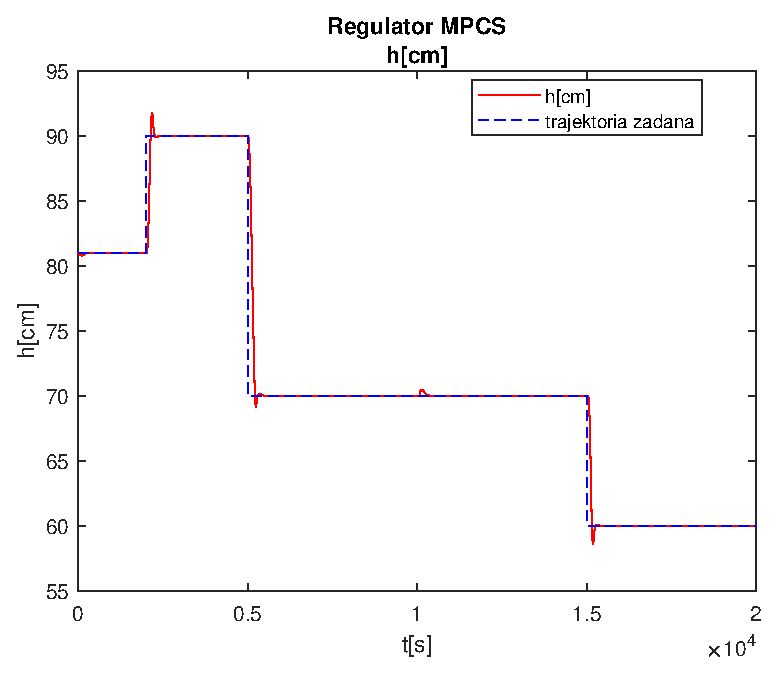
\includegraphics[width=1\linewidth]{img/MPCSanaLin/MPCSLinHN300Nu100l10.eps}
      \caption{}
      \label{fig:fig:MPCSLinN300Nu100l101}
   \end{subfigure}
       
   \begin{subfigure}[b]{0.4\textwidth}
      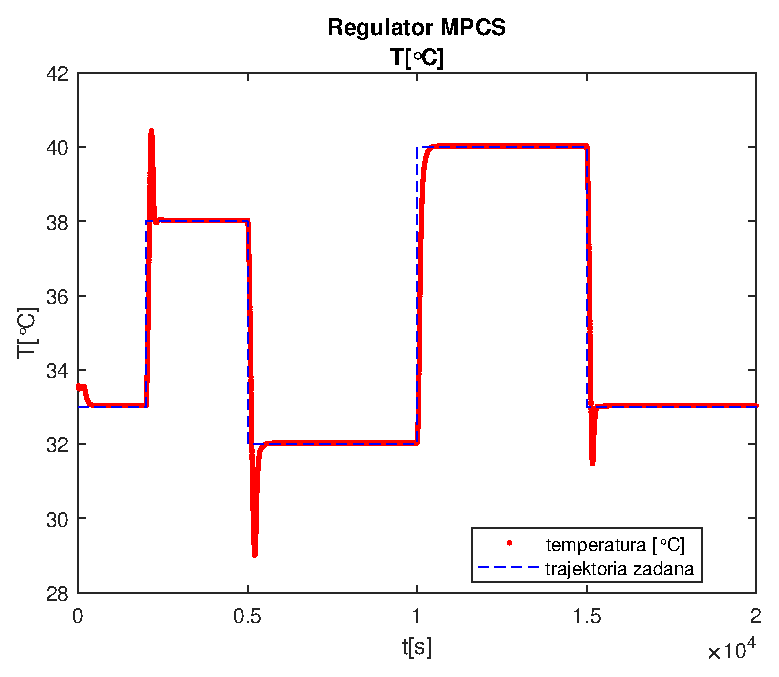
\includegraphics[width=1\linewidth]{img/MPCSanaLin/MPCSLinTN300Nu100l10.eps}
      \caption{}
      \label{fig:fig:MPCSLinN300Nu100l102}
   \end{subfigure}
       
   \begin{subfigure}[b]{0.4\textwidth}
      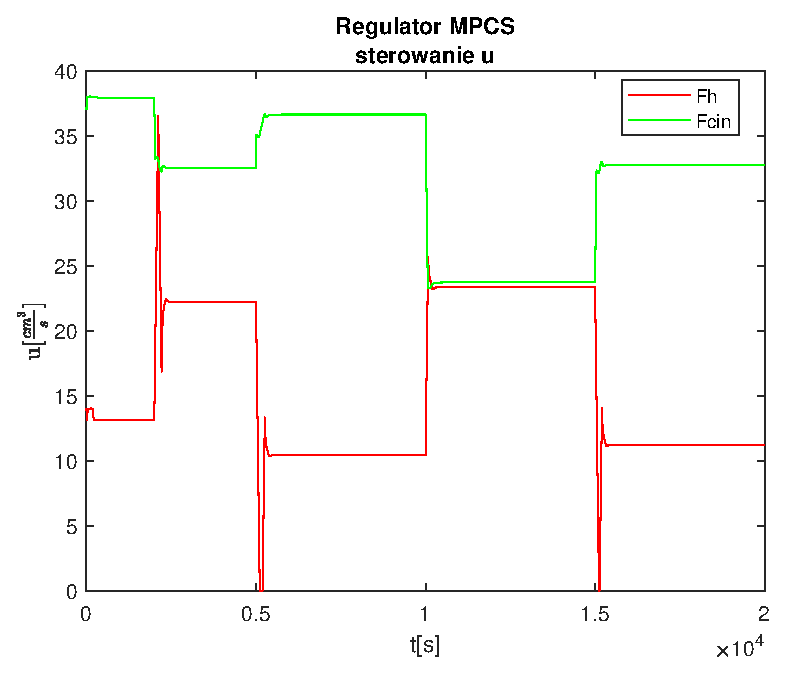
\includegraphics[width=1\linewidth]{img/MPCSanaLin/MPCSLinControlN300Nu100l10.eps}
      \caption{}
      \label{fig:fig:MPCSLinN300Nu100l103}
   \end{subfigure}
       
   \caption{Wykresy dla regulatora MPCS, obiekt nieliniowy.}
   \label{fig:MPCSLinN300Nu100l10}
\end{figure}
           
